\begin{figure}\centering
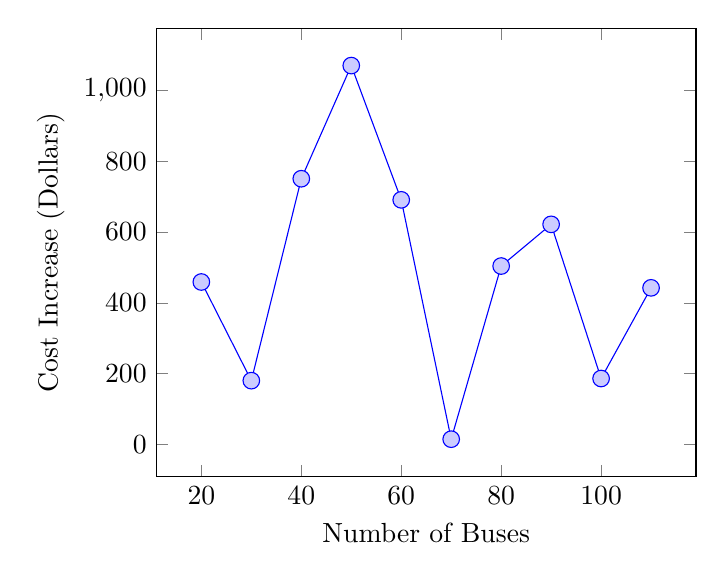
\begin{tikzpicture}
\begin{axis}[xlabel=Number of Buses, ylabel=Cost Increase (Dollars), legend pos=north west]
	\addplot[blue] coordinates {
	  (20, 14312.58/10 - 9724.43/10)  
		(30, 16113.51/10 - 14312.58/10)  
		(40, 23617.81/10 - 16113.51/10)
		(50, 34317.80/10 - 23617.81/10)  
		(60, 41226.07/10 - 34317.80/10)  
		(70, 41374.21/10 - 41226.07/10) 
		(80, 46412.54/10 - 41374.21/10)  
		(90, 52628.26/10 - 46412.54/10)
		(100, 54490.15/10 - 52628.26/10) 
		(110, 58912.91/10 - 54490.15/10 )}; 
\addplot[blue!20, draw=blue, only marks, mark size=3pt] coordinates {
    (20, 14312.58/10 - 9724.43/10)  
		(30, 16113.51/10 - 14312.58/10)  
		(40, 23617.81/10 - 16113.51/10)
		(50, 34317.80/10 - 23617.81/10)  
		(60, 41226.07/10 - 34317.80/10)  
		(70, 41374.21/10 - 41226.07/10) 
		(80, 46412.54/10 - 41374.21/10)  
		(90, 52628.26/10 - 46412.54/10)
		(100, 54490.15/10 - 52628.26/10) 
		(110, 58912.91/10 - 54490.15/10 )}; 
\end{axis}
\end{tikzpicture}
\caption{Cost comparison for different numbers of buses}
\label{fig:results:scalabilityRuntimes}
\end{figure}
